

\documentclass[main.tex]{subfiles}

\begin{document}

\chapter{Tensile response of brittle-matrix composites}
\label{LEC:TensileResponse}

The appearance of disintegration mechanisms introduced in the previous lectures was describing the material and structural behavior in view of the damage and failure mechanisms. In the present chapter, however, we will focus on a phenomenon appearing in brittle-matrix composites that uses the interaction between emerging cracks and debonding of the reinforcement form the matrix to achieve a desired structural behavior. The concept of tension-stiffening is well known in steel-reinforced concrete. It can be further exploited when using non   

\section{Pseudo-ductility}

Tensile response of a reinforced specimen can be regarded as
dynamically evolving chain of crack bridges. 
Cracks emerging during the tensile loading of a reinforced concrete specimen
act as starting points of debonding. The structural behavior of the system
can be describing by regarding two inelastic mechanisms - cracking and 
an adjacent debonding. To understand the principle concept how to achieve ductile behavior 
using purely elastic-brittle components, let us use a simple analytical description
of the cracking and debonding process.

The response of fibrous composites to tensile loading depends on the material properties of both the matrix, and the fibers, and their interface \cite{cox:52,marcoxeva:85,cur:93c}. The typical form of such a response includes an initial linear stage with the stiffness defined by the rule of mixtures as
\begin{equation}
 \Ec = \Ef \Vf + \Em(1-\Vf)
\label{eqn:Ec}
\end{equation}
with $\Ef$ and $\Em$ denoting the fiber and matrix moduli of elasticity, respectively, and $\Vf$ denoting the fiber volume fraction. With the inception of the first matrix crack marking the beginning of multiple cracking (matrix fragmentation), the stiffness starts to decrease. During the following phase of multiple cracking, stress redistributions both between and within the constituents take place. This second phase continues up to the state where all fibers are fully debonded so that the composite is saturated with cracks, which marks the start of the third phase -- a linear response with stiffness equal to $\Ef\Vf$. The vertical offset between the composite stress in the third phase and an equivalent reinforcement response $\Ef\Vf\epsc$, with $\epsc$ being the global strain, is due to the tensile stress accumulated in the matrix fragments (see Fig.~\ref{FIGTensileResponse}).


Probabilistic approach to modeling of composites exhibiting fragmentation in one of the components with has been applied by several authors in the past, e.g. \cite{avekel:73,huiphoibn:95}.
The class of methods generally referred to as ``random strength approach'' \cite{casgellac:10}
can be informally explained using the graphical representation of stress states at several selected load levels shown in Fig.~\ref{FIGMutipleCracking}. The matrix strength distribution shown in all diagrams was simulated by a random field following the Weibull probability distribution.

The first diagram (Fig.~\ref{FIGMutipleCracking}a) shows the matrix stress along the specimen after the first crack has appeared at the location of minimum matrix strength. Upon further loading, the matrix stress is growing until the matrix strength has been is reached at some other point of the specimen (Fig.~\ref{FIGMutipleCracking}b). New crack is then inserted into the numerical representation of the specimen by updating the stress profile (Fig.~\ref{FIGMutipleCracking}b) in accordance with the considered crack bridge model summarized in Fig.~\ref{FIGSingleCrackBridge}.

The crack bridge model delivers the local profile of the matrix stress in the vicinity of the crack. The stress profile depends on the underlying bond law describing the stress transfer between the reinforcement and the matrix and on the instantaneous crack spacing. In the shown example a simple crack bridge model with constant bond has been used. For this model, expressions for matrix stress ($\sigma_\mathrm{m}$), reinforcement strain ($\varepsilon_\mathrm{f}$), and of crack width $w$ required by the crack-tracing algorithm are available in a closed form as summarized in Fig.~\ref{FIGSingleCrackBridge}.

%
\begin{equation} \label{eq: simple_cb_stress}
\sigma_{\mathrm{m}}=
\begin{cases}
\dfrac{TV_{\mathrm{f}}}{1-V_{\mathrm{f}}}|z|  & : |z|<a \\
\dfrac{\sigma_\mathrm{c} E_{\mathrm{m}}}{E_{\mathrm{m}}(1-V_{\mathrm{f}})+E_{\mathrm{f}}V_{\mathrm{f}}} & : |z| \ge a
\end{cases}
\end{equation}
where $z$ is the local coordinate equal to zero at the crack bridge position, $T$ is the bond intensity, $V_{\mathrm{f}}$ is fiber volume fraction, $\sigma_\mathrm{c}$ is the composite stress, and $E_{\mathrm{f}}$, $E_{\mathrm{m}}$ denote the stiffness of the reinforcement and of the matrix, respectively.
The instantaneous debonded length $a$ is given as the product of the remote stress and bond intensity $a = T \sigma_{\mathrm{c}}$.
The resulting linear matrix strain profiles $\varepsilon_{\mathrm{m}} = \sigma_{\mathrm{m}} / E_{\mathrm{m}}$ and $\varepsilon_{\mathrm{f}} = (\sigma_{\mathrm{c}} - \sigma_{\mathrm{m}} ) / E_{\mathrm{f}}$ in the vicinity of a crack bridge are depicted in Fig.~\ref{FIGSingleCrackBridge}b. The grey area represents the crack opening $w = \int (\varepsilon_{\mathrm{f}} - \varepsilon_{\mathrm{m}}) \, \mathrm{d}z$.

This model has already been derived in Sec.~\ref{SEC:PullOutAnalytical} for one-sided pull-out for rigid matrix. An extension for elastic matrix using an additional kinematic equation has been provided in Sec.~\ref{SEC:PullOutAnalyticalElasticMatrix}. 

With the detected cracks, stress and strain profiles and values of crack openings at hand, the nominal composite strain can be evaluated. The process of crack detection, stress update and strain evaluation is repeated until the saturated crack state has been achieved. The simulation delivers the relation between the composite stress and strain as shown in Fig.~\ref{FIGMutipleCracking}e. At the same time, the matrix crack widths in all crack bridges is evaluated at individual levels of composite stress; see Fig.~\ref{FIGMutipleCracking}f. This detailed output allows the user to analyze the sensitivity of the composite behavior to the input parameters and their statistical variability. Parameters used for the present example are summarized in Fig.~\ref{fig:example}e. Although the matrix stress profiles show a 100~mm long composite, the stress-strain diagram and the crack widths were simulated for a composite with a length of 3000~mm.

\paragraph{Composite stress-strain curve}
With the identified history of the matrix cracking states $K = 1,2,\ldots, K_{\mathrm{sat}}$ at hand, the composite strains $\epsc$ corresponding to the load $\load$ can be evaluated for the given crack positions $\pmb{X}^{(K)}$ as
\begin{equation}
\epsc^{(K)}(\load) =
\frac{1}{\Lc} \left[
\sum_{k=1}^{K} \CMOD_k^{(K)}(\load) +
\frac{1}{\Em} \int\limits_{0}^{\Lc} \sigmam^{(K)}(\load,x)\,\mathrm{d}x
\right].
\label{eq:avg_strain}
\end{equation}
The matrix stress $\sigmam^{(K)}$ is prescribed by Eq.~(\ref{eqn:matrix_stress_general}) and the $K$ crack openings $\CMOD_k^{(K)}$, $k=1,2,\dots,K$ have to be provided by a crack bridge model.


\begin{figure}
    \centering
        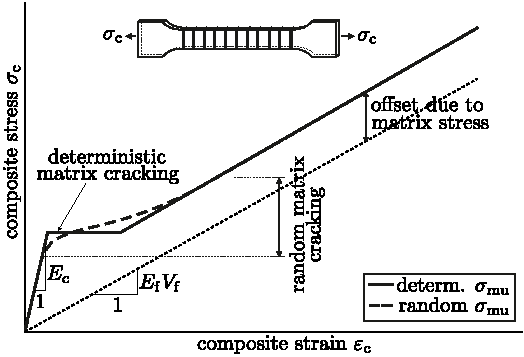
\includegraphics[width=10cm]{fig/rand_determ_matrix.pdf}
        \caption{Tensile response of a composite specimen, random, deterministic matrix}
        \label{FIGTensileResponse}
\end{figure}



\begin{figure}
    \centering
        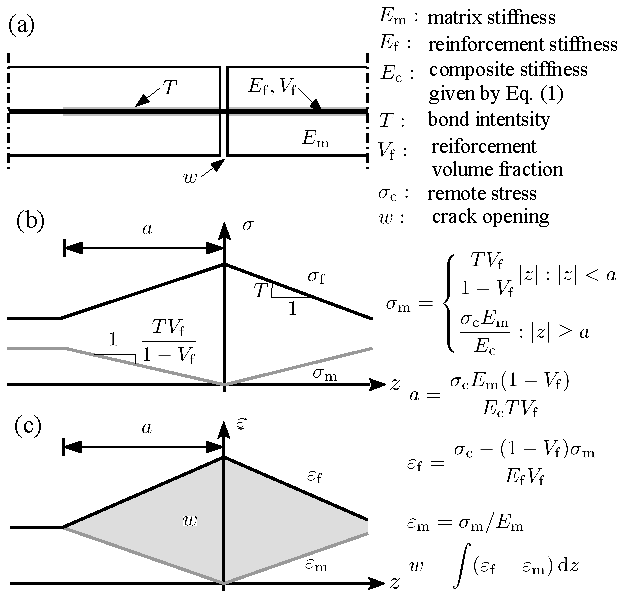
\includegraphics[width=10cm]{fig/simple_crack_bridge.pdf}
        \caption{Stress and strain state of a single crack bridge with constant bond}
        \label{FIGSingleCrackBridge}
\end{figure}


\begin{figure}
    \centering
        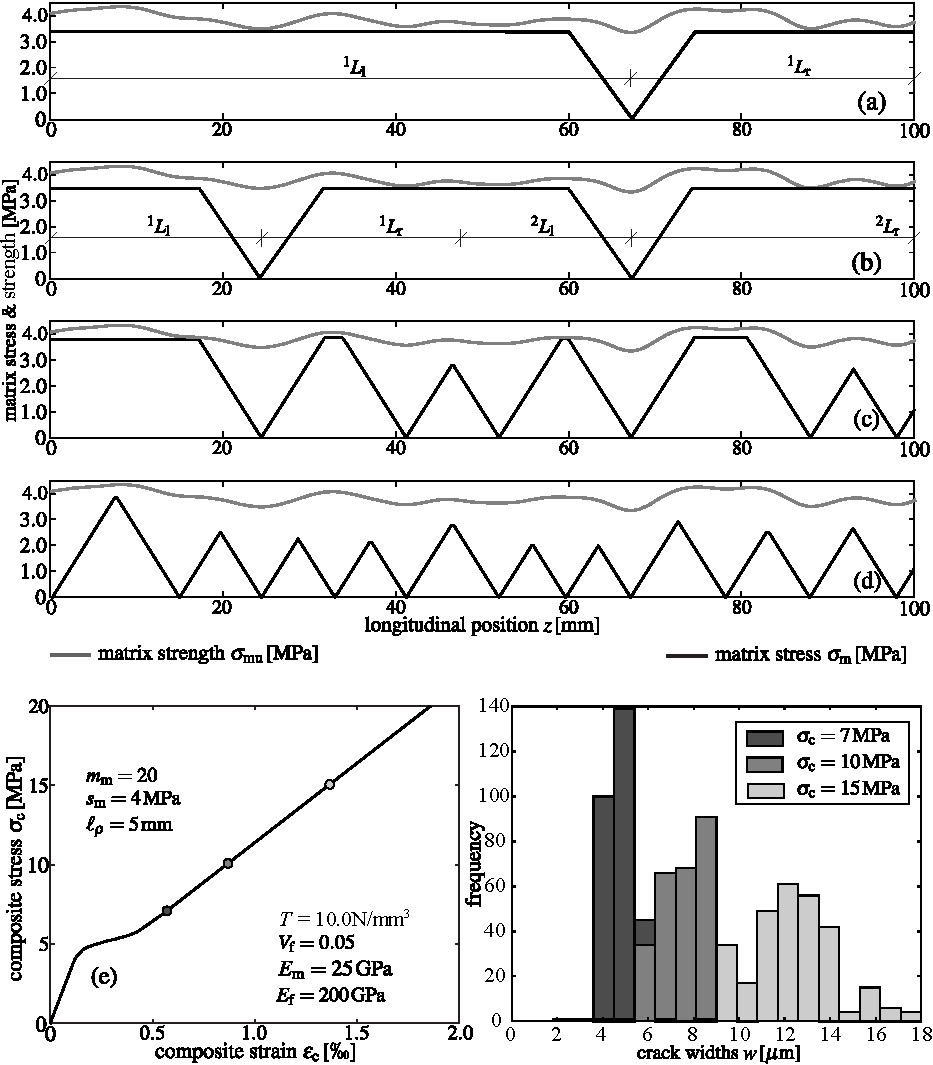
\includegraphics[width=10cm]{fig/crack_evolution.pdf}
        \caption{Stress and strain state along the tensile specimen at increasing remote stress levels}
        \label{FIGMutipleCracking}
\end{figure}

\subsection{Effect of reinforcement ratio}

Given the strain hardening curve

\begin{align}
    \label{}
\end{align}

\end{document}


\begin{itemize}
\item Crack as a starting point of delamination
\item Multiple cracking, using finite elements? alternative approaches?
\item Statistics – just a sugar?
\item Characterization strategies
\item Measurement techniques
\item Modeling approaches
\end{itemize}

\chapter{Influence of heterogeneity}

Seminars – with focus on application to
\begin{itemize}
\item Steel-reinforced concrete
\item Textile-reinforced concrete
\item Short-fiber concrete
\item Ceramics composites
\end{itemize}


\chapter{Shear loading}

Interaction of fibers and matrix.
Layers
